\chapteruaf{Using Page Allocation Timings to Detect VMI}


\section{Motivation}\tabularnewline
In this chapter we discuss a simple statistical analysis of the time taken to map a page in main memory. When we look at resources shared between the Host and the Guest one of the most obvious ones is main memory. In the x86-64 processor main memory by the Memory Management Unit (MMU), which uses a process called paging to control which data and instructions are held in main memory. 

When a VMI program is used on a guest memory is mapped from the memory space of the guest to the memory space of the host (which, for brevity, we will refer to as guest-space and host-space respectively). We believe this mapping from guest-space to host-space will affect which pages are in memory to a degree that is measurable in the time required to map a page in memory.  


\section{Experimental Design}

For our initial experiment we aim to determine whether or not a guest VM can detect that it is being monitored by a VMI process. We begin by using the same experimental hardware described in chapter 2.  For our experimental setup we use a KVM and a Xen host. Each host runs a single VM of Ubuntu 14.04 as described in chapter II.  

On the host the VMI agent was run continuously. We did three trials: one where the process-list command was run, one where the module-list command was run, and one where the map-addr command was run. In each case the VMI program is continually run on the guest VM. 


On the guest side a probe is set up. This probe uses the C++11 chrono object~\cite{_chrono_2014} which gives us nanosecond resolution. For each iteration the time stamp is recorded, a page is mapped and unmapped from memory using the mmap function~\cite{_mmap2_2014}, and then the timestamp is again recorded. The difference between the second time stamp and the first time stamp are taken and this result is recorded as the time taken to map and unmap a page. As mentioned earlier however a small correction is made and the overhead time in the previous section is subtracted from the result to give our final result.  A control sample where no VMI agent is being run on the guest is also taken. 


\begin{enumerate}\label{MMapAlg}
	\item Mark Timestamp $t_0$
	\item map page in memory
	\item unmap page in memory
	\item Mark Timestamp $t_1$
	\item Record $t_1$-$t_0$
\end{enumerate}

\section{Analysis}

The first step of our analysis is to compare the histograms of the control data with data here VMI is used.  It can be seen immediately (figs ~\ref{XenMMapHist1} and ~\ref{KVMMMapHist1}) that not only are the samples with VMI different from the control sample but they are also different f
rom each other as well. One should note that these histograms are zoomed in to give a better insight into the data. There are still small pockets of data after the 10,000ms bin but these are so small as to be not evident in the histograms.  The next step is to determine whether or not these datasets are statistically different from the data in the control sample. To do this we use two statistical tests, which determine whether or not two populations share the same mean. The first is Welch's t-test ~\cite{welch_generalization_1947} which determines whether the mean of two populations is the same. The second is the Mann Whitney U-test which again measures whether the two means of the population are the same.


	\begin{figure}[ht]\label{XenMMapHist1}
	  \centering
	  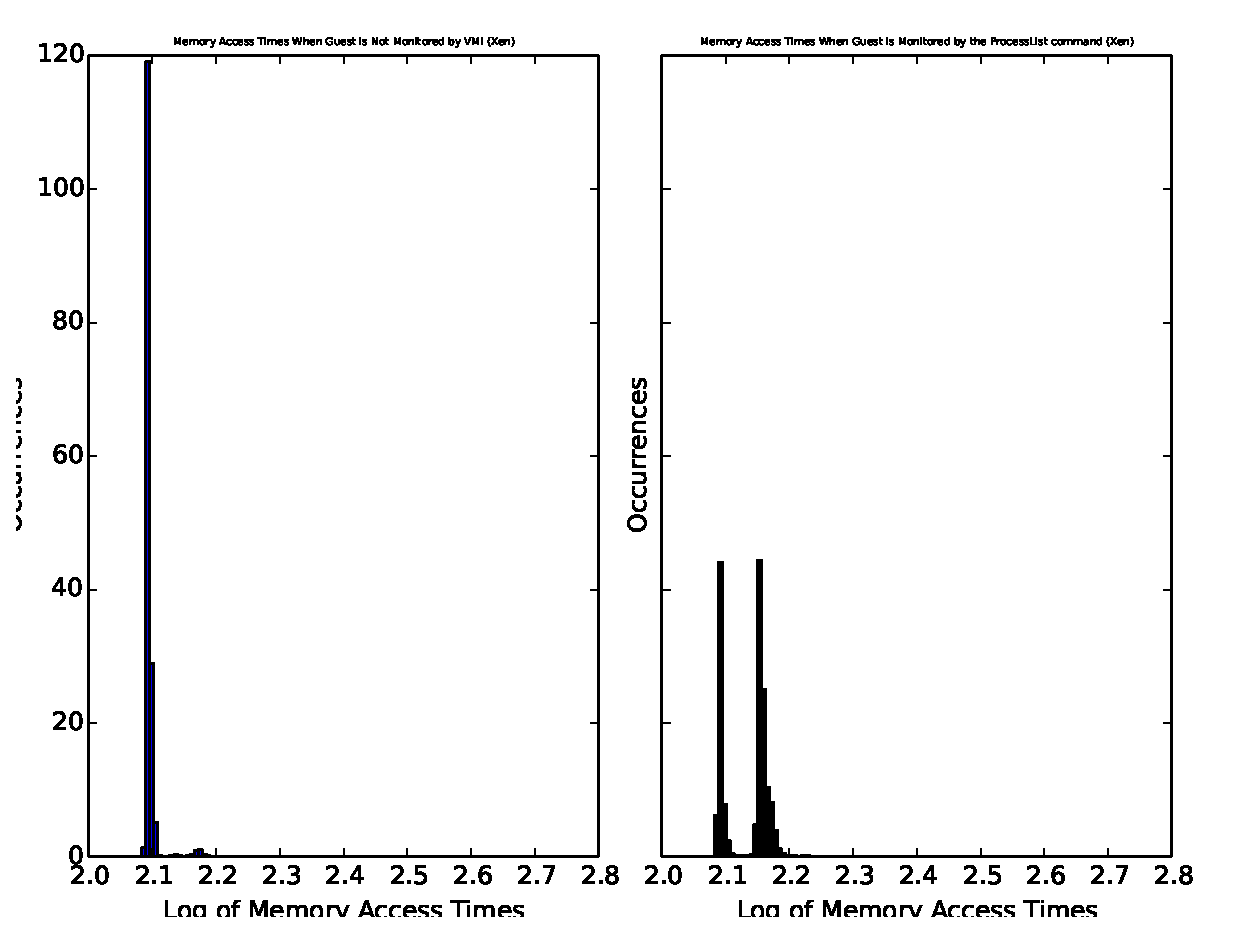
\includegraphics[width=\textwidth]{figures/XenNoVMIVsProcList.eps}
	  \caption{Histograms of the log of mmap time when a Xen VM is not observed by VMI (left) and observed by the process-list command (right)}
	\end{figure}


	\begin{figure}[ht]\label{KVMMMapHist1}
	  \centering
	  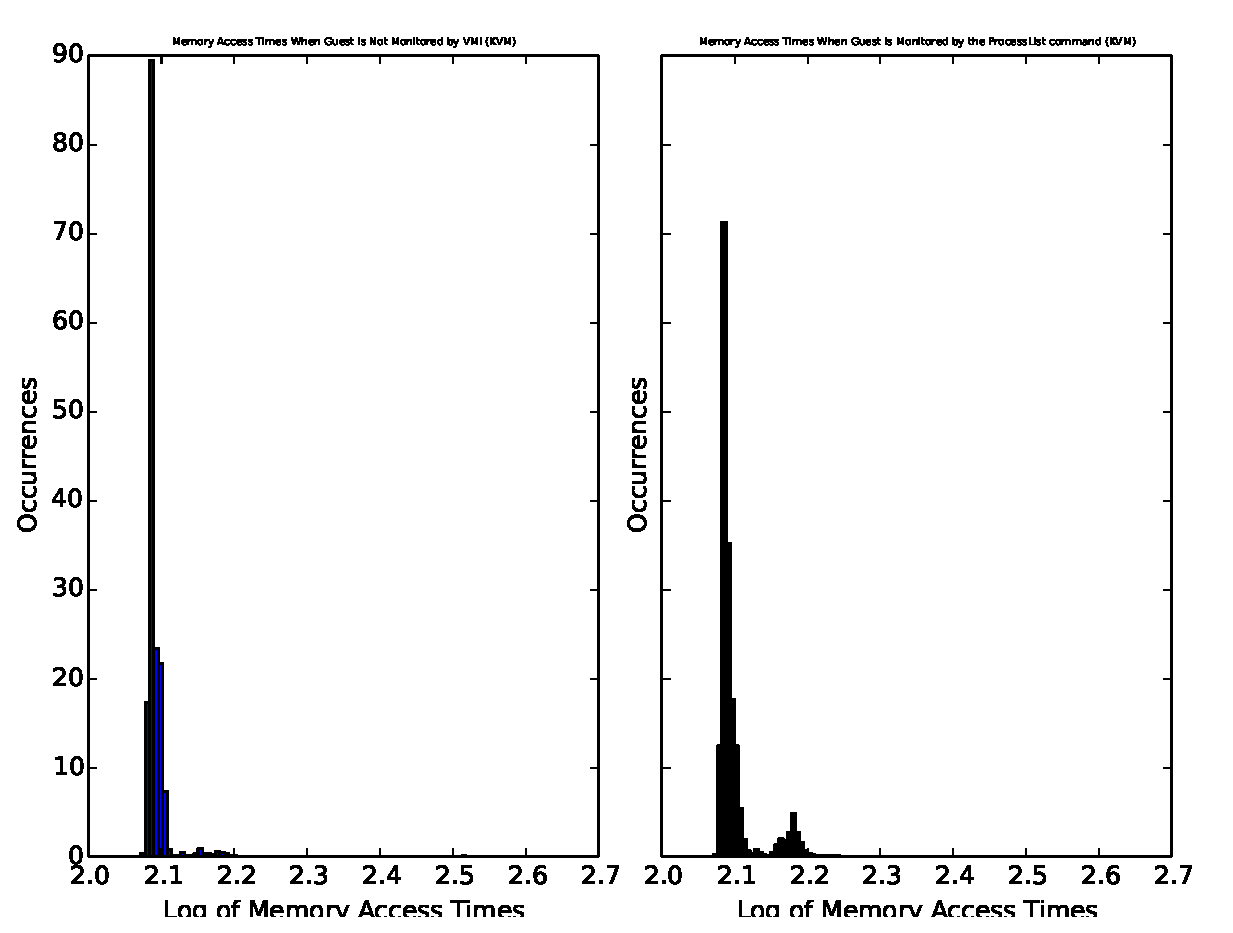
\includegraphics[width=\textwidth]{figures/KVMMMApTestNoVMIvsProcList.eps}
	  \caption{Histograms of the log of mmap time when a KVM VM is not observed by VMI (left) and observed by the process-list command (right)}
	\end{figure}

In both cases we begin with the null hypothesis that the mean of a sample not being monitored by VMI is the same as the mean of a sample which was being monitored by some form of VMI. The results of these tests are shown in table ~\ref{TStatsMMap1}. 
As we can see the results of the likelihood of the means of the two populations being is extremely low. It should be noted here that while all of the p-values are 0 this is strictly speaking not possible for finite populations. Instead this is a limitation of IEEE floating point arithmetic and a value of 0 should be taken as a value of less than  . 


The next question to arise is this are these patterns unique to VMI or can they be reproduced by other means? To answer this we first consider which factors can impact time taken to map a page are page faults and cache misses~\cite{bryant_computer_2003}.  At the scale of time being dealt with in this experiment cache misses will likely not be a significant factor given that they tend to operate in the 100ns range. As a result we will instead focus on page faults. 


	\begin{table}
		\centering
		\begin{tabular}{| c | c | c | c |}
			\hline
			Hypervisor & mapPage & modList & procList  \\ \hline
			Xen & -4361 & -5678 & -1691  \\  \hline
			KVM & -903 & -1000 & -632  \\ \hline

		\end{tabular}
		\label{TStatsMMap1}
		\caption{T stats for Xen and KVM compared to the null hypothesis that no VMI is being used}
	\end{table}



For our first experiment we will test whether a VM with more memory will cause a similar patterns in the mmap timings to a VM  being monitored by a VMI agent. We test our control data against data taken from a clone of our VM only with 4GB of RAM instead of 1GB. Again the VM is idle except for the probe running and no VMI used on the VM. We get the following results (figs tables). 

<insert tables and figs>


We can see that they are distinctly different. We then compare them to those taken by the control VM being monitored by VMI. We can see from these results (figs tables) that the memory timings are different when compared to our timings taken when the VM is being monitored by VMI.

<insert tables figs> 


Next we test to see whether the number of VMs being run can be confused with the use of VMI on a VM. In this experiment we begin by adding an identical clone of our control VM and then running the probe on the control VM. We then repeat the process adding a 3rd and 4th VM. VMs are labeled A,B,C, and D (figure) and have identically allocated resources. 

We first compare the results of this experiment to those derived from using some form of VMI using our statistical tests (table). We can see from those tests that when multiple VMs are run on the same host a different signature in the MMap timings is produced compared to when the VM is being monitored by VMI.  We then in the interest of being thorough perform a test where two VMs are being run simultaneously on the same physical host. We then do the same VMI continuously monitor one of the two VMs with 

This is contrary to the expected result in which the amount of time required to map a page increases for each VM added. 